\newpage
\section{Aufbau}

Der Aufbau der Versuche zur Bestimmung des Schubmoduls G und des magnetischen Moments besteht hauptsächlich aus zwei Elementen.

\begin{figure}[h]
  \centering
  \includegraphics[height=8cm]{Grafiken/Magnetfeld.pdf}
  \caption{Versuchsapparatur\cite{1}.}
  \label{fig:Versuch}
\end{figure}

Der erste Bestandteil ist die Messappatur aus Abb.: 4, an der der Torsionsdraht über ein Justierrad an einer Klemmschraube fixiert ist.
Am anderen Ende des Drahtes ist eine Kugel durch eine Schraube befestigt.
Zur Messung des magnetischen Momentes wird zusätzlich ein Helmholtzspulenpaar benötigt, welches an eine konstante Stromquelle angeschlossen ist.
Im Zentrum des Spulenpaares befindet sich die Kugel, in deren Inneren sich ein Permanentmagnet befindet.
An dem Torsionsdraht über der Kugel ist ein ebener Spiegel angebracht.

\begin{figure}[h]
  \centering
  \includegraphics[height=4.5cm]{Grafiken/Periodendauermessung.pdf}
  \caption{Schematische Darstellung der Periodendauermessung.}
  \label{fig:Periodendauer}
\end{figure} 

Der zweite Teil des Aufbaus wird in Abb.: 5 dargestellt.
Hier wird das Licht einer Lampe durch einen Spalt und eine Sammellinse auf den gerade beschriebenen Spiegel gebündelt.
Falls der Lichtstrahl in einem bestimmten Winkel von dem Spiegel reflektiert wird, trifft dieser auf einen Lichtdetektor.
Durch den Lichtdetektor und eine digitale Schaltung, die in Abbildung 6 dargestellt ist, wird das optische Signal in ein elektrisches Signal umgewandelt und an eine elektronische Uhr weitergeleitet.

\begin{figure}[h]
  \centering
  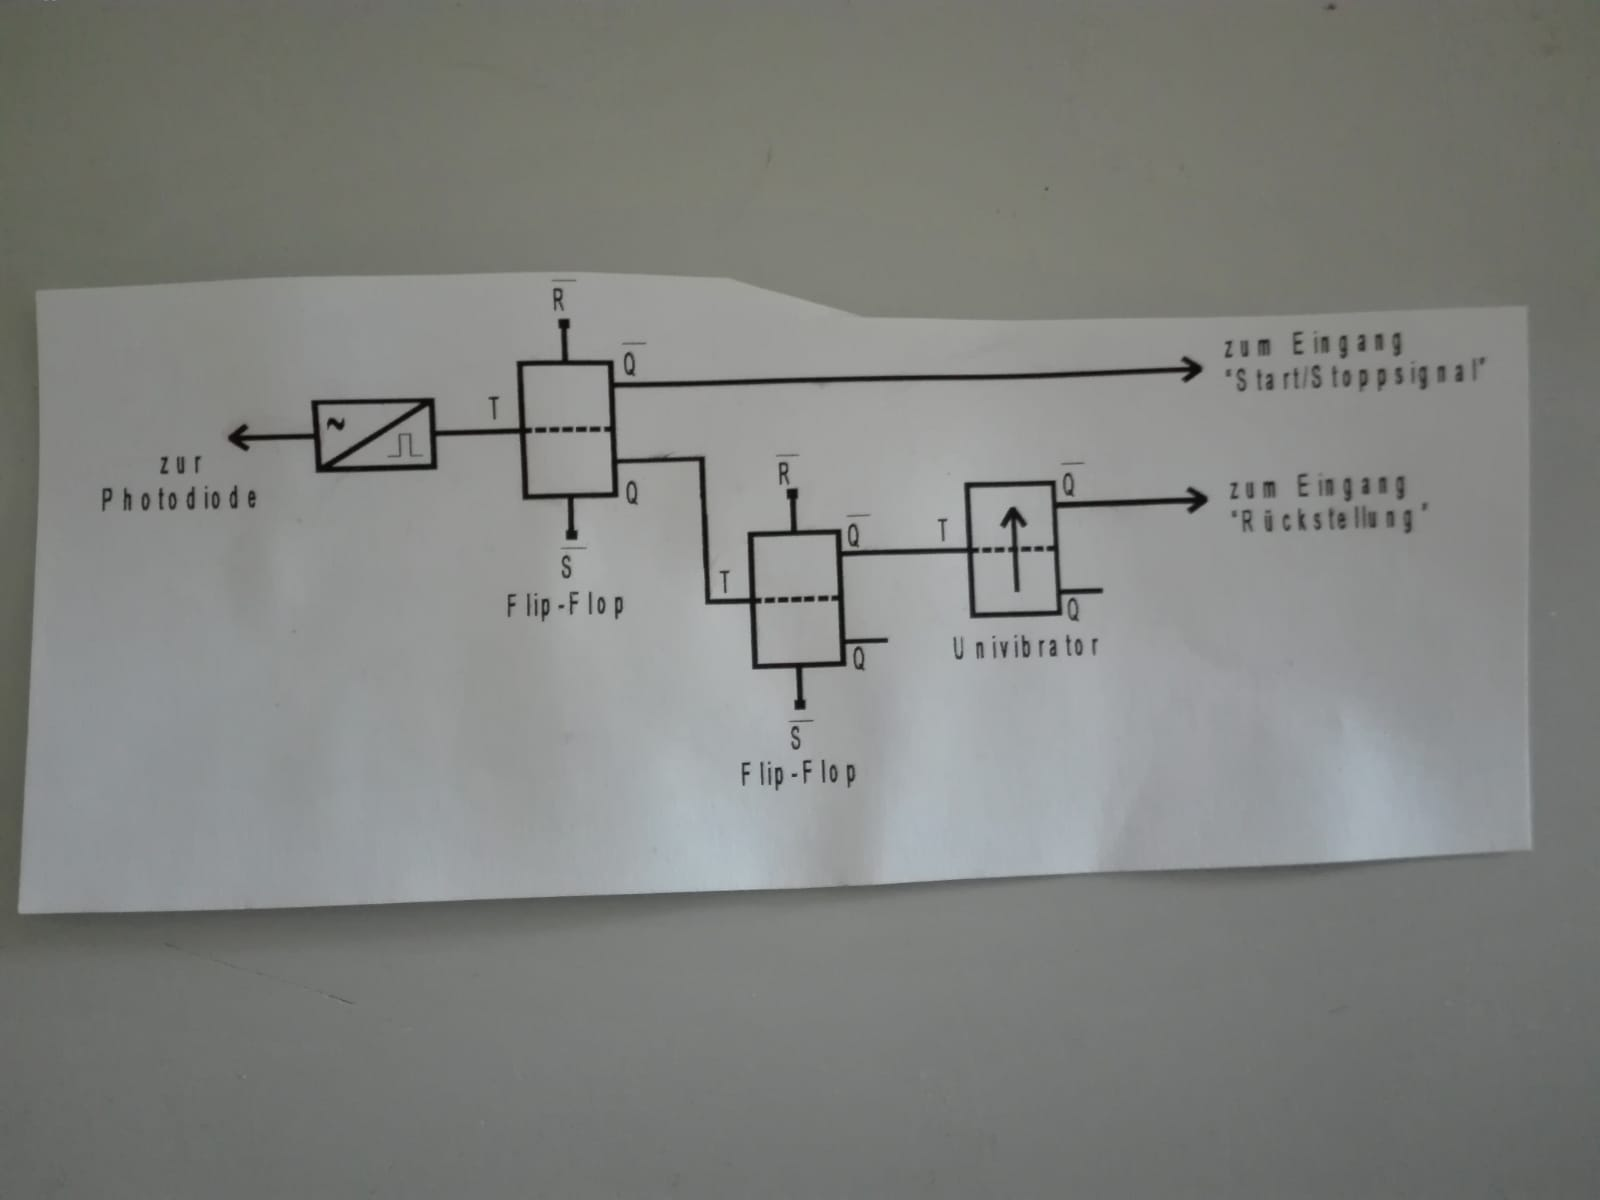
\includegraphics[height=5cm]{Grafiken/Schaltung foto.jpg}
  \caption{Schematischer Aufbau der Schaltung}
  \label{fig:Schaltung}
\end{figure} 



